\documentclass{5220hw}
\usepackage{amsmath,amssymb,latexsym, mathtools}
\usepackage{verbatim}
\usepackage{algorithm}
\usepackage{algpseudocode}
\usepackage{changepage}

\algnewcommand\Or{\textbf{or}}
\setlength{\parindent}{1cm}

\begin{document}

\name{Sheroze Sheriffdeen}
\netid{mss385}

\maketitle

\begin{exercises}

\item A given program spends 10\% of its time in an initial startup phase, and then 90\% of its time in work that can be easily parallelized.  Assuming a machine with homogeneous cores, plot the idealized speedup and parallel efficiency of the overall code according to Amdahl's law for up to 128 cores.  If you know how, you should use a script to produce this plot, with both the serial fraction and the maximum number of cores as parameters.

Amdahl's Law: 
\begin{equation}
S(p) = \dfrac{1}{ \alpha + \frac{1}{p} (1 - \alpha)}
\end{equation}

where $S(n)$ is the speedup, $n$ is the number of cores, $B$ is the fraction of code that is strictly serial. In our example, $\alpha$ is 0.1. Then, the speedup as a function of the number of cores is as follows.

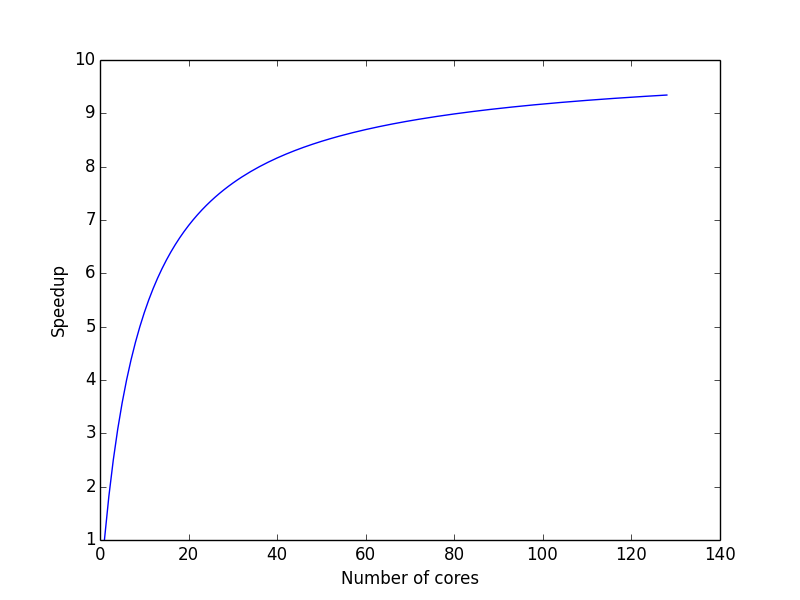
\includegraphics[scale=0.7]{speedup.png}

\item Suppose a particular program can be partitioned into perfectly independent tasks, each of which takes time $\tau$.  Tasks are set up, scheduled, and communicated to $p$ workers at a (serial) central server; this takes an overhead time $\alpha$ per task. What is the theoretically achievable throughput (tasks/time)?

To complete $p$ tasks, the setups takes $\alpha p + \tau$ time. $\alpha p$ time to distribute the work and $\tau$ time to complete the work in parallel. Therefore, the throughput is, 
\begin{equation}
	T = \dfrac{p}{ \alpha p + \tau }
\end{equation}

\item Under what circumstances is it best to not tune?

\begin{itemize}
	\item When the time contributed to the effort to tune exceeds the time saved by tuning.
	\item When the bottlenecks of performance have not been identified.
	\item When a review of the underlying algorithm has not been performed to improve performance.
\end{itemize}

\item The class cluster consists of eight nodes and fifteen Xeon Phi accelerator boards.  Based on an online search for information on these systems, what do you think is the theoretical peak flop rate (double-precision floating point operations per second)?  Show how you computed this, and give URLs for where you got the parameters in your calculation.  (We will return to this question again after we cover some computer architecture.)

According to the Intel calculations, the theoretical peak flop rate for a single Xeon Phi 5110p coprocessor is,
16 FLOPS/clock x 60 cores x 1.053 GHz = 1010.88 GF/s.
\footnote{https://www-ssl.intel.com/content/www/us/en/benchmarks/server/xeon-phi/xeon-phi-theoretical-maximums.html}

According to the Intel spec,\footnote{http://download.intel.com/support/processors/xeon/sb/xeon\_E5-2600.pdf} the peak flop rate for the Intel Xeon E5-2620 v3 processors is 120GF/s. 

We have 15 Xeon Phis and $8 * 12$ Intel Xeon E5-2620 v3 processors leading to a, \\
$1010.88 * 15 + 96 * 120 = 26.68$ TF/s of total theoretical peak flop rate.

\item What is the approximate theoretical peak flop rate for your own machine?

I have a Mid 2014 Retina MacBook Pro. It has a Intel Core i5-4278U processor with a base frequency of 2.6 GHz and two cores. The flop rate is then 2 * 2.6 = 5.2 GF/s.

\end{exercises}

\end{document}
